% ------------------------------------
% Universidad de Costa Rica
% Facultad de Ingeniería
% Escuela de Ingeniería Eléctrica
% IE0499 - Proyecto Eléctrico
%
% PLANTILLA DEL TRABAJO ESCRITO
% ------------------------------------

% Tipo de documento
\documentclass[]{proyectoelectrico}

% A. PAQUETES Y MACROS ESPECIALES -------
% Aquellos que no están incluidos en la clase
% proyectoelectrico.cls

% -----------------------------------------
% OTROS PAQUETES E INSTRUCCIONES ESPECIALES
% -----------------------------------------

% Para insertar código fuente estilizado
\usepackage{listings}
	\lstset{basicstyle=\ttfamily,
    		breaklines=true,
            numbers=left, 
    		numberstyle=\tiny, 
    		stepnumber=1, 
    		numbersep=6pt}

% Para insertar símbolos extraños
\usepackage{marvosym}

% Para insertar texto fútil
\usepackage{lipsum}

% NUEVAS INSTRUCCIONES

\newcommand{\EIEx}{\textsc{Escuela \Lightning~ Ingeniería Eléctrica}}

% Definición de algunos símbolos matemáticos
\newcommand{\me}{\mathrm{e}}
\newcommand{\mi}{\mathrm{i}}
\newcommand{\mj}{\mathrm{j}}
\newcommand{\md}{\mathrm{d}}
\usepackage{libertine}
%\usepackage{libertinust1math}
\usepackage[T1]{fontenc}
\renewcommand*{\ttdefault}{cmtt}

% B. DATOS ------------------------------
% Todos los nombres incluyen dos apellidos
% y acentos y signos de puntuación apropiados.

% Título del proyecto
\titulo{Diseño de una readecuación eléctrica del edificio del Planetario de la Universidad de Costa Rica}

%% Autor (nombre y carné)
\autor{Luis Alberto Salazar Romero}
\carne{B36359}

% Profesor(a) guía
\guia{Ing. Irene Víquez Barrantes}

% Profesores lectores 
\lectorA{Ing. Osvaldo Fernandez Cascante}
\lectorB{Ing. Jorge Sanchez Monge}

% Fecha de entrega del trabajo escrito
\mes{5}
\ano{2018}

% ------------------------------------

%%%%%%%%%%%%%%%%%%%
\begin{document}
%%%%%%%%%%%%%%%%%%%

\frontmatter

% 1. PORTADA
\portada

% 2. HOJA DE APROBACIÓN
\aprobacion

% 3. RESUMEN
% --------------------------------
% EL RESUMEN
% ----------

\begin{resumen}{Diseño eléctrico, Planetario, Seguridad humana, Iluminación}

Este proyecto consiste en la elaboración de un diseño eléctrico del planetario de la Universidad de Costa Rica incluyendo los cálculos, planos y especificaciones técnicas necesarias para que cada uno de los sistemas diseñados funcione apropiadamente. Este proyecto propone específicamente una readecuación de los sistemas de iluminación y de seguridad humana de dicha edificación, ya que se considera que el resto de los sistemas actualmente en funcionamiento fueron dimensionados apropiadamente, por lo cual no propician disconformidad en los usuarios. 

\end{resumen}
% EL RESUMEN EN INGLÉS
% --------------------

\begin{theabstract}{Electrical Retrofitted design of Costa Rica’s University Planetarium building}{Electrical design, Planetarium, Human security, Lighting}

This project consists in the elaboration of an electrical design of the Costa Rica’s University Planetarium Building, including the calculations, plans and technical specifications that are necessaries for each of the designed systems to work properly. This project proposes specifically a readjustment on lighting and human security systems currently built, because it is considered that the rest of the systems in operation are currently appropriately sized, and doesn't imply users inconvenience.

\end{theabstract}



%\begin{resumen}{Diseño eléctrico, Planetario, Seguridad humana, Iluminación}
%	
%	Este proyecto consiste en la elaboración de un diseño eléctrico del planetario de la Universidad de Costa Rica incluyendo los cálculos, planos y especificaciones técnicas necesarias para que cada uno de los sistemas diseñados funcione apropiadamente.
%	
%	 Este proyecto propone específicamente una readecuación de los sistemas de iluminación y de seguridad humana de dicha edificación, ya que se considera que el resto de los sistemas actualmente en funcionamiento fueron dimensionados apropiadamente, por lo cual no propician disconformidad en los usuarios. 
%	
%\end{resumen}

% 4. DEDICATORIA
% LA DEDICATORIA
% --------------

\begin{dedicatoria}
Dedicado a mi padre el Ing. Jorge Alberto Salazar G.
\end{dedicatoria}

% 5. AGRADECIMIENTOS
%% LOS AGRADECIMIENTOS
% -------------------

\begin{agradecimientos}

A don Erick y al profesor Leonardo por su gran colaboración como encargados del planetario de la Universidad de Costa Rica durante todo el proyecto. Al Arq. Kevin Cotter Murillo por facilitarme los planos eléctricos actuales de la edificación. A la Ing. Irene Víquez Barrantes por tenderme una mano y su guía durante este proceso. A los ingenieros Osvaldo Fernandez Cascante y Jorge Sanchez Monge por brindarme sus observaciones y sugerirme mejoras para este proyecto.

\end{agradecimientos}

% 6. TABLAS DE CONTENIDO, FIGURAS Y TABLAS
% ----------------------------------------
\tableofcontents
%\listoffigures
\listoftables

% 7. NOMENCLATURA
% ---------------
% LA NOMENCLATURA
% ---------------

\mainmatter

% 8. CAPÍTULOS
% ------------
% ----------------------
  \chapter{Introducción}
% ----------------------
\label{C:introduccion}

Este proyecto nace de la inquietud de los encargados del Planetario de la Universidad de Costar Rica respecto a deficiencias en el sistema de iluminación. Además al estudiar más detalladamente el proyecto se pudo constatar notables carencias y deficiencias en los sistemas de seguridad humana como lo son el sistema de detección de incendios, el sistema de alarmas contra robo y la ausencia de un sistema de vigilancia de circuito cerrado de televisión (CCTV). Debido a esto, se propone realizar un diseño eléctrico de este edificio ajustado a las necesidades reales de los usuarios, de modo que represente la base para una futura remodelación eléctrica del mismo. Dicho diseño consiste en la elaboración de los cálculos, planos y especificaciones técnicas necesarias para que cada uno de los sistemas diseñados funcione apropiadamente.

%- sección ----------------------------------------------------------


\section{Alcance del proyecto}

El alcance de este proyecto se limita específicamente al diseño de una readecuación de los sistemas de iluminación y de seguridad humana del planetario de la Universidad de Costa Rica, ya que se considera que el resto de los sistemas actualmente en funcionamiento fueron dimensionados apropiadamente, por lo cual propician disconformidad en los usuarios. Por último se propone la realización de un cambio en los modelos de los tomacorrientes por un aspecto meramente estético, pero no es parte del alcance de este proyecto la reubicación, ni el cálculo de protecciones, ni el dimensionamiento del cableado y la canalización para este sistema.

\section{Objetivos}

\vspace{0.4cm}

\subsection{Objetivo general}
Diseñar los planos eléctricos y especificaciones técnicas necesarios para satisfacer las necesidades actuales en materia eléctrica y de seguridad humana del Planetario de la Universidad de Costa Rica en una futura remodelación. 

\subsection{Objetivos específicos}
Para el desarrollo de este proyecto se establecieron los siguientes objetivos:

\begin{enumerate}
	\item Realizar un levantamiento de la condición eléctrica actual del edificio.
	\item Realizar un estudio de iluminación del edificio.
	\item Elegir los equipos eléctricos y de seguridad humana que mejor se ajusten a las necesidades del proyecto.
	\item Diseñar la ubicación de los equipos eléctricos y de seguridad humana que se van a instalar en la edificación.
	\item Realizar un estudio de la carga a instalar.
	\item Realizar los cálculos necesarios para que los sistemas diseñados funcionen correctamente.
	\item Elaborar los planos constructivos en formato .DWG.
	\item Elaborar las especificaciones técnicas del proyecto.
\end{enumerate}

\section{Metodología}
La metodología utilizada debe listarse en forma cronológica.

El desarrollo del trabajo incluyó los siguientes pasos y procedimientos, listados en secuencia:

\begin{enumerate}
	\item Solicitud de los planos eléctricos actuales del planetario de la Universidad de Costa Rica a la Oficina Ejecutora del Programa de Inversiones de la Universidad de Costa Rica (OEPI).
	\item Revisión de sitio contra planos suministrados por la OEPI sobre la condición eléctrica actual del edificio.
	\item Realización de un estudio de iluminación del edificio mediante el uso del software DIALux considerando los pasillos como sala de exhibición.
	\item Elección de los modelos de luminarias más adecuados utilizando como referencia los valores de luminosidad proporcionados por el software DIALux y comparándolos con los modelos de luminarias LED del catálogo 2017 de Sylvania.
	\item Realización de una pequeña investigación acerca de los estándares y marcas de equipos de seguridad humana que utiliza la Universidad de Costa Rica.
	\item Elección de los equipos de seguridad humana que mejor se ajusten a las necesidades del proyecto tomando en cuenta los estándares y marcas que utiliza la Universidad de Costa Rica.
	\item Elaboración de una propuesta y dibujo en formato .DWG de la ubicación de las luminarias y equipos de seguridad humana que se van a instalar en la edificación.
	\item Realización un estudio de la carga eléctrica nueva a instalar, tomando en cuenta la que se eliminará.
	\item Elaboración del cálculo de las protecciones y dimensionamiento de cableado y canalización necesarios para la instalación de los equipos nuevos. Se incluye un nuevo cálculo de las acometidas en caso de ser necesaria su sustitución.
	\item Realización de una reubicación de los equipos propuestos a instalar en caso de tener que eliminar algunos por condiciones de carga eléctrica.
	\item Elaboración final de los planos constructivos en formato .DWG incluyendo las ubicaciones finales de los equipos.
	\item Redacción las especificaciones técnicas del proyecto, incluyendo las marcas, modelos y certificaciones permitidas para los materiales, métodos y condiciones de instalación de dichos equipos. Se agregará toda aquella información que se considere necesaria para la óptima conclusión del proyecto.
\end{enumerate}

%\section{Desarrollo o contenido}
%Como último párrafo de la introducción, debe indicarse al lector lo que se presenta en el informe, con una breve descripción del contenido de cada capítulo, mostrando la secuencia lógica de estos.


% ----------------------
  \chapter{Marco Teórico} 
% ----------------------
\label{C:antecedentes}


\section{Sistema de iluminación}

\subsection{Normativa}

La normativa que se debe seguir para el diseño de sistemas de iluminación según el articulo 1 del decreto No 36979-MEIC es la normativa NFPA 70. \cite{CIEMI}




\subsection{Estudio de iluminación}

Consiste en estudiar y analizar las condiciones de iluminación artificial de un sitio en $lux$, bajo ciertas condiciones de operación y luz ambiente.

\subsubsection{DIALux}


Es un software gratuito en sistema operativo Windows para el cálculo, diseño y visualización de la luz de manera profesional. El software es utilizado por más de 700 000 diseñadores en todo el mundo. Además se puede diseñar utilizando los catálogos de luminarias de los principales fabricantes del mundo y permite superponer los datos de CAD de otros programas arquitectónicos para el diseño de iluminación requerido. \cite{DIALux}


\subsubsection{Recomendaciones de niveles de iluminación}

La exposición prolongada al exceso o escasez de iluminación en un lugar puede causar repercusiones en la salud, ya sea a nivel visual o una lesión debido a no poder observar claramente cuando se está realizando una actividad, por lo cual el Instituto de Normas Técnicas de Costa Rica fija en su norma INTE 31-08-06-2000 los parámetros mínimos de iluminación requeridos para una actividad en especifica. (Ver apendice \ref{A}) \cite{Inteco}\\
 



\subsection{Tecnologías de iluminación}

Las tecnologías de iluminación varían dependiendo de la fuente de luz. \cite{Syl}
 
\subsubsection{Diodo Emisor de Luz (LED)}

\begin{itemize}
	
	\item Altamente eficientes (hasta 130-150 lúmenes por watt).
	
	\item Bajo consumo ( alrededor del 40-80\% que fuentes de luz incandescente).
	
	\item Baja temperatura de operación.
	
	\item Ecológicas y 100\% reciclables.
	
	\item Durables (entre 25 000 y 50 000 horas de vida útil).
	
	\item Alta variedad de dimensiones y aplicaciones.
	
\end{itemize}


\subsubsection{Fluorescente}


\begin{itemize}
	
	\item Bajo consumo ( 80\% menos que las lámparas incandescentes).
	
	\item Alta duración (hasta diez veces mayor que las luminarias incandescentes).
	
	\item Alto rendimiento de color y eficiencia lumínica.
	
\end{itemize}



\subsubsection{Incandescente y Halógeno}


\begin{itemize}
	
	\item Bajo costo.
	
	\item Altos índices de reproducción cromática
	
	\item Ideal para ambientes que busquen confort y relajamiento.
	
\end{itemize}


\subsubsection{Alta Intensidad de Descarga (HID)}


\begin{itemize}
	
	\item  Alto flujo luminoso.
	
	\item Ideal para parqueos, naves industriales, canchas deportivas, entre otros.
	
	\item Alto grado de fidelidad de color.
	
	\item Alta eficacia.
	
	\item Larga vida útil.
	
\end{itemize}

\subsubsection{Aditivos Metálicos Cerámicos (CMI)}

\begin{itemize}
	
	\item Alto rendimiento de color.
	
	\item Ideal para tiendas y comercios.
	
\end{itemize}




\subsection{Carga continua}

Se define como carga cuya corriente máxima se prevé que circule durante tres horas o más. (100.1) \cite{NFPA70}


\subsection{Carga no continua}

Se define como carga cuya corriente máxima se prevé que circule durante menos de tres horas. (100.1) \cite{NFPA70}


\subsection{Circuito ramal}

Se define como conductores de circuito entre el dispositivo final contra sobre-corriente que protege el
circuito y las salidas.(100.1) \cite{NFPA70}

\subsection{Interruptor automático}

Se define como un dispositivo diseñado para que abra y cierre un circuito de manera no automática,pero que abra el circuito automáticamente cuando se produzca una sobre-corriente predeterminada, sin daños para sí mismo cuando alcance su valor nominal. (100.1) \cite{NFPA70}


\subsection{Interruptor automático contra falla a tierra (GFCI)}

Se define como un dispositivo, que funciona desenergizando un circuito o parte de éste dentro de un período de tiempo determinado, cuando una corriente a tierra supera los valores establecidos para un dispositivo de Clase A. (100.1) \cite{NFPA70}


\subsection{Interruptor automático contra falla de arco (AFCI)}

Se define como un dispositivo destinado a brindar protección contra los efectos de falla de arco desenergizando el circuito cuando se detecten las características únicas de la formación del arco. (210.12(A))\cite{NFPA70}



\subsection{Cálculo protecciones en circuitos ramales}


El valor nominal de la protección contra sobre-corriente para cargas continuas y no continuas o cualquier combinación de ambas debe ser menor a la carga no continua más el 125\% de la carga continua. (210.20(A)) \cite{NFPA70} \\

\textbf{Excepción:} cuando todos los dispositivos del circuito ramal incluida su protección contra sobre-corriente, estén listados para su funcionamiento al 100\% de su valor nominal, se permitirá que el valor nominal del dispositivo de sobre-corriente no sea menor que la suma de la carga continua más la carga no continua.


\subsection{Cálculo del calibre de cable en circuitos ramales}

El calibre de cable debe calcularse según su ampacidad y valor máximo de temperatura permitido, de acuerdo con lo establecido en el articulo 310.16. (ver apéndice \ref{B}) \cite{NFPA70}


%\subsection{Tipos de aislamiento de cable}




\newpage




\section{Sistema de alarmas contra incendio}


\subsection{Normativa}

La normativa que se debe seguir para el diseño de sistemas de alarmas contra incendio según el Cuerpo de Bomberos de Costa Rica es la normativa NFPA 72. \cite{Bomberos}


\subsection{Tipos de fuego}

Cuando ocurre un incendio este se debe a la combustión de ciertos materiales, clasificando los tipos de fuego en: \cite{Bomberos}\\

\begin{itemize}
	
	\item \textbf{Clase A:} 
	
\begin{itemize}
	\item \textbf{Material combustible:} combustibles comunes como madera, tela, papel, caucho y plásticos.
\end{itemize}
	
	
	\item \textbf{Clase B:} 

\begin{itemize}
	\item \textbf{Material combustible:} líquidos y gases inflamables como aceites, grasas,
	alquitranes, base de pinturas y lacas.
\end{itemize}	


	\item \textbf{Clase C:} 

\begin{itemize}
	\item \textbf{Material combustible:} equipos eléctricos energizados.
\end{itemize}



	\item \textbf{Clase D:} 

\begin{itemize}
	\item \textbf{Material combustible:} metales como magnesio, titanio, zirconio, sodio, litio, potasio entre otros.
\end{itemize}

	\item \textbf{Clase K:} 

\begin{itemize}
	\item \textbf{Material combustible:} utensilios o materiales de cocina como aceites minerales, animales y grasas.
\end{itemize}

	
	
\end{itemize}


\subsection{Dispositivos de iniciación ó detección de incendio}


Son los dispositivos del sistema que se encargan de censar constantemente las condiciones del ambiente en busca de indicios de incendio. Estos dispositivos o sensores pueden ser direccionales o no, es decir que pueden indicar la locación o zona del incendio o bien solo activar el sistema. El fuego tiene ciertas características que pueden ser censadas y dar indicios de incendio, tales como humo, llama, calor, entre otros. (3.3.122) \cite{NFPA72} 

\subsubsection{Detectores de humo}

Son aquellos dispositivos que detectan como indicio de incendio partículas de humo visible o invisible. Estos varían según su aplicación y tiempo de respuesta. (3.3.59.19)

\begin{itemize}
	
	\item \textbf{Detector por cámara de niebla:} utiliza un dispositivo fotoeléctrico para medir la densidad de una muestra de aire dentro de la recamara del sensor, si la densidad de la muestro original es variada debido a la presencia de partículas de humo el sensor entra en condición de alarma. (3.3.252.1)
	
	
	\item \textbf{Detector por ionización:} utiliza un material radiactivo para ionizar el aire entre dos electrodos, cuando existe presencia de partículas de humo estas causan que el flujo de iones decrezca y el sensor entre en condición de alarma si cumple con los parámetros establecidos. (3.3.252.2)
	
	
	\item \textbf{Detector por efecto fotoeléctrico de obstrucción:} utilizan una fuente de luz y un foto-receptor no enfocado, al entrar humo en el sensor este dispersa la luz produciendo que parte de esta llegue al foto-receptor quien evaluara dicha dispersión y dará condición de alarma si cumple con los parámetros establecidos. (3.3.252.3)
	
	\item \textbf{Detector por efecto fotoeléctrico de dispersión:} utilizan una fuente de luz y un foto-receptor enfocado, al entrar humo en el sensor este dispersa la luz produciendo que disminuya la cantidad de luz que llega al foto-receptor quien evaluara dicha dispersión y dará condición de alarma si cumple con los parámetros establecidos. (3.3.252.4)

	\item \textbf{Detector por imagen de video:} utiliza técnicas de análisis de imagen en tiempo real para detectar la presencia de humo. (3.3.252.5)
	
	\item \textbf{Detector por haz proyectado:} utiliza una fuente de luz, un foto-receptor y un espejo, cuando hay presencia de partículas de humo entre el haz de luz y el espejo, este dispersa la luz que llega al foto-receptor produciendo la señal de alarma. (3.3.59.15)

	\item \textbf{Detector en ducto de aire acondicionado:} responde ante al censado de partículas de humo en el sistema de aire acondicionado. (17.7.4)	
	
	\item \textbf{Detector de muestreo de aire:} consiste en una red de tuberías que van desde el detector hasta las áreas a proteger. El detector aspira aire de la zona a proteger y lo hace correr a través de la red de tuberías pasando por varios puestos de muestreo para detección de humo. (3.3.59.1)
		

\end{itemize}


\subsubsection{Detectores de gas por fuego}

Consiste en dispositivo que detecta gases producidos por fuego como $CO_{2}$, $CO$, $N_{2}$, $H_{2}$, entre otros. (3.3.59.6)


\subsubsection{Detectores de energía radiante}

Consiste en un dispositivo capaz de censar la energía radiante como ultravioleta, visible o infrarrojo. (3.3.59.16)


\begin{itemize}
	
	\item \textbf{Detector de llama:} dispositivo capaz de censar la energía radiante producida por grandes llamas. (3.3.59.8)
	
	\item \textbf{Detector de chispas y brasas:} dispositivo capaz de censar la energía radiante producida por chispas y brasas. Generalmente utilizado en lugares oscuros y en el rango de infrarrojo. (3.3.59.8)
	
\end{itemize}



\subsubsection{Detectores de calor}

Consiste en un dispositivo capaz de censar la temperatura, la taza de cambio de la temperatura o ambos de un lugar determinado. (3.3.59.9)


\begin{itemize}
	
	\item \textbf{Detector por conductividad eléctrica:} utiliza una resistencia que varía en función de la temperatura. (3.3.59.5)
	
	\item \textbf{Detector de temperatura fija:} responde cuando su elemento operativo se calienta a una temperatura determinada. (3.3.59.7)
	
	\item \textbf{Detector con tubería de tasa de incremento neumático:} consiste en una serie de tuberías de pequeñas de cobre que se instalan en el techo y los muros. El tubo termina en un detector que contiene diafragmas y contactos configurados para actuar a una presión predeterminada. El sistema es lo suficientemente robusto para aceptar los pequeños cambios de temperaturas normales. (3.3.59.14)
	
	\item \textbf{Detector de tasa de compensación:} responde cuando la temperatura del aire que rodea el dispositivo alcanza un nivel determinado. (3.3.59.17)
	
	\item \textbf{Detector de incremento:} responde cuando la tasa de incremento en la temperatura supera un valor determinado. (3.3.59.18)
	
\end{itemize}
 
 
\subsubsection{Detectores de flujo} 
 
Consiste en un sensor que monitorea el flujo en la tubería de supresión de incendio, si hay un cambio en el flujo de la tubería por más de 90 segundos igual o superior al rociador más pequeño instalado, se envía señal de alarma. (17.12.2)
 

\subsubsection{Detectores multi-criterio}

Consiste en un dispositivo con múltiples sensores que responden por separado ante un estímulo físico como calor, humo, gases de combustión, entre otros. El detector envía una única señal de alarma, ya sea por la activación de uno de los sensores o varios de ellos. Este dispositivo tiene la capacidad de priorizar su censado según su aplicación. (3.3.59.11)   


\subsubsection{Estaciones manuales}

Es un dispositivo utilizado manualmente para iniciar la señal de alarma de incendio. (3.3.8.3)



\subsection{Dispositivos de notificación de incendio}

Consisten en dispositivos que por medio de luces, bocinas, táctil o mensajes escritos informan el estado de alarma y la ruta de evacuación a las personas dentro de la zona de riesgo. (3.3.160)\cite{NFPA72}

\subsubsection{Notificación audible}

Consiste en la notificación utilizando el sentido de la audición, generalmente mediante el uso de sirenas y  bocinas. (3.3.160.1)


\begin{itemize}
	
	\item \textbf{Notificación audible de salida:} utiliza el sentido de la audición con el fin de guiar a las personas en riego a la salida más cercana, se utiliza para rutas de evacuación o reubicación. (3.3.160.1.1)
	
	\item \textbf{Notificación audible de texto:} utiliza un mensaje pre-gravado para informar a las personas en riego el estado de alarma, además brinda indicaciones y medidas de seguridad. (3.3.160.1.2)
		
\end{itemize}


\subsubsection{Notificación táctil}

Consiste en un dispositivo que alerta por medio del sentido del tacto o la vibración. (3.3.160.2)

\subsubsection{Notificación visual}

Consiste en un dispositivo que alerta por medio del sentido de la vista. (3.3.160.3)


\begin{itemize}
	
	\item \textbf{Notificación visual de salida:} utiliza el sentido de la vista con el fin de guiar a las personas en riego a la salida más cercana, se utiliza para rutas de evacuación o reubicación, generalmente luces estroboscópicas. (3.3.160.3)
	
	\item \textbf{Notificación visual de texto:} utiliza un mensaje visual para informar a las personas en riego el estado de alarma, además brinda indicaciones y medidas de seguridad, típicamente monitores y pantallas. (3.3.160.3.1)
	
\end{itemize}



\subsection{Dispositivos de control}

Son todos aquellos dispositivos que se utilizan con opciones de control y monitoreo específicamente.


\subsubsection{Unidad de control o panel de control de alarma}


Es un dispositivo del sistema provisto de fuentes de energía primaria y secundaria, con entradas capaces de recibir señales de los dispositivos de iniciación u otros dispositivos y procesarlas para determinar que funciones requeridas en cada una de sus salidas. (3.3.92)\cite{NFPA72}\\

El panel de control debe cumplir al menos uno o varias de las siguientes funciones: (23.3.3.1)


\begin{enumerate}
	
	\item Iniciación manual de señal de alarma.
	
	\item Alarma contra incendio automática y señal de supervisión.
	
	\item Monitoreo de condiciones de falla en sistemas de supresión.
	
	\item Activación de los sistemas de supresión.
	
	\item Activación de los sistemas de seguridad.
	
	\item Activación de los dispositivos de notificación.
	
	\item Activación de sistemas de voceo de emergencia.
	
	\item Servicios de supervisión del departamento de seguridad.
	
	\item Monitoreo del departamento de seguridad.
	
	\item Activación de señales fuera de las instalaciones.
	
	\item Combinación de sistemas.
	
\end{enumerate}

 
\subsubsection{Módulo de monitoreo}

Es un dispositivo que proporciona la dirección específica de otros dispositivos de iniciación no direccionables como contactos magnéticos u otros dispositivos de seguridad mediante el monitoreo con cableado de conexiones normalmente cerradas o normalmente abiertas de contactos secos.\cite{Monitoreo}


\subsubsection{Módulo de relé}

Es un dispositivo utilizado para funciones de control como descenso del ascensor, apagado del aire acondicionado, entre otros. El estado del relé se comunica requiriendo solo una dirección de dispositivo.\cite{Rele}

\subsubsection{Módulo de aislamiento}

Es un dispositivo capaz de aislar las comunicaciones direccionables para mejorar la conveniencia de la instalación y aumentar la integridad del sistema. El aislamiento se activa automáticamente cuando se detecta un cortocircuito en la salida. También se puede seleccionar el aislamiento manualmente desde el panel de control para ayudar a solucionar los problemas de cableado.\cite{MAislamiento}


%\subsection{Fuentes de poder}



%
%
%10.5.6.3* Capacity.
%
%10.5.6.3.1 The secondary power supply shall have sufficient
%capacity to operate the system under quiescent load (system
%operating in a nonalarm condition) for a minimum of
%24 hours and, at the end of that period, shall be capable of
%operating all alarm notification appliances used for evacuation
%or to direct aid to the location of an emergency for 5 minutes,
%unless otherwise permitted or required by the following:
%
%(1) Battery calculations shall include a 20 percent safety mar-
%gin to the calculated amp-hour rating.
%(2) The secondary power supply for in-building fire emer-
%gency voice/alarm communications service shall be ca-
%pable of operating the system under quiescent load for a
%minimum of 24 hours and then shall be capable of oper-
%ating the system during a fire or other emergency condi-
%tion for a period of 15 minutes at maximum connected
%load.
%(3) The secondary power supply capacity for supervising sta-
%tion facilities and equipment shall be capable of support-
%ing operations for a minimum of 24 hours.
%(4) The secondary power supply for high-power speaker ar-
%rays used for wide-area mass notification systems shall be
%in accordance with 24.4.3.4.2.2.
%(5) The secondary power supply for textual visible appliances
%shall be in accordance with 24.4.3.4.7.1.
%(6) The secondary power supply capacity for central control sta-
%tions of a wide-area mass notification systems shall be ca-
%pable of supporting operations for a minimum of 24 hours.
%(7) The secondary power supply for in-building mass notifica-
%tion systems shall be capable of operating the system un-
%der quiescent load for a minimum of 24 hours and then
%shall be capable of operating the system during emer-
%gency condition for a period of 15 minutes at maximum
%connected load.
%10.5.6.3.2 The secondary power supply capacity required
%shall include all power supply loads that are not automatically
%disconnected upon the transfer to secondary power supply.
%10.5.6.4 Secondary Power Operation.
%10.5.6.4.1 Operation on secondary power shall not affect the
%required performance of a system or supervising station facility,
%including alarm, supervisory, and trouble signals and indications.
%10.5.6.4.2 Systems operating on secondary power shall com-
%ply with Section 10.17.
%10.5.6.4.3 While operating on secondary power, audio ampli-
%fier monitoring shall comply with 10.17.2.1.2.
%10.5.7* Continuity of Power Supplies.
%10.5.7.1 The secondary power supply shall automatically pro-
%vide power to the protected premises system within 10 seconds
%whenever the primary power supply fails to provide the mini-
%mum voltage required for proper operation.
%10.5.7.2 The secondary power supply shall automatically pro-
%vide power to the supervising station facility and equipment
%within 60 seconds whenever the primary power supply fails to
%provide the minimum voltage required for proper operation.
%10.5.7.3 Required signals shall not be lost, interrupted, or
%delayed by more than 10 seconds as a result of the primary
%power failure.
%
%10.5.7.3.1 Storage batteries dedicated to the system or UPS
%arranged in accordance with the provisions of NFPA 111, Stan-
%dard on Stored Electrical Energy Emergency and Standby Power Sys-
%tems, shall be permitted to supplement the secondary power sup-
%ply to ensure required operation during the transfer period.
%10.5.7.3.2 Where a UPS is employed in 10.5.7.3.1, a positive
%means for disconnecting the input and output of the UPS sys-
%tem while maintaining continuity of power supply to the load
%shall be provided.
%



%
%23.18.2 Power Supplies. A primary battery (dry cell) shall be
%permitted to be used as the sole power source of a low-power
%radio transmitter where all of the following conditions are met:
%(1) Each transmitter shall serve only one device and shall be
%individually identified at the receiver/fire alarm control
%unit.
%(2) The battery shall be capable of operating the low-power
%radio transmitter for not less than 1 year before the bat-
%tery depletion threshold is reached.
%(3) A battery depletion signal shall be transmitted before the
%battery has been depleted to a level below that required to
%support alarm transmission after 7 additional days of non-
%alarm operation. This signal shall be distinctive from
%alarm, supervisory, tamper, and trouble signals; shall vis-
%ibly identify the affected low-power radio transmitter;
%and, when silenced, shall automatically re-sound at least
%once every 4 hours.
%(4) Catastrophic (open or short) battery failure shall cause a
%trouble signal identifying the affected low-power radio
%transmitter at its receiver/fire alarm control unit. When
%silenced, the trouble signal shall automatically re-sound at
%least once every 4 hours.
%(5) Any mode of failure of a primary battery in a low-power
%radio transmitter shall not affect any other low-power ra-
%dio transmitter




\subsection{Tipos de cableado}

Para los sistemas de alarmas contra incendio existen los siguientes tipos de lazos o cableado: (12.3)\cite{NFPA72}\\


\begin{itemize}
	
	\item \textbf{Clase A}:  (12.3.1)
	
	\begin{enumerate}
		
		\item Incluye redundancia.
		
		\item La capacidad operativa continúa más allá de una única apertura.
		
		\item Se anuncian las condiciones que afectan la operación prevista de la ruta.
		
	\end{enumerate}
	
	\item \textbf{Clase B}: (12.3.2)
	
	\begin{enumerate}
	
	\item No incluye redundancia.
	
	\item La capacidad operativa se detiene en una única apertura.
	
	\item Se anuncian las condiciones que afectan la operación prevista de la ruta.
	
	\end{enumerate}	
	
	\item \textbf{Clase C}: (12.3.3)
	
	\begin{enumerate}
	
	\item Incluye una o más rutas en las que la capacidad operativa se verifica a través de una comunicación de extremo a extremo, pero la integridad de las rutas individuales no se controla.
	
	\item Se anuncia una pérdida de comunicación de extremo a extremo.
	
	\end{enumerate}	
	
	\item \textbf{Clase D}: (12.3.4)
	
	\begin{enumerate}
	
	\item Tiene una operación a prueba de fallas, no se anuncia ningún fallo, pero la operación prevista se realiza en caso de una falla en la ruta.
	
	\end{enumerate}	
	
	\item \textbf{Clase E}: (12.3.5)
	
	\begin{enumerate}
	
	\item No es monitoreada por integridad.
	
	\end{enumerate}	



	\newpage
	
	

	
	\item \textbf{Clase X}: (12.3.6)
	
	\begin{enumerate}
	
	\item Incluye redundancia.
	
	\item La capacidad operativa continúa más allá de una única apertura o cortocircuito.
	
	\item Se anuncian las condiciones que afectan la operación prevista de la ruta.
	
	\end{enumerate}	
	
\end{itemize}

También es importante mencionar que el cableado para aplicaciones tradicionales es el siguiente:

\begin{itemize}
	
	\item \textbf{Circuitos de iniciación (IDC):} clase A y clase B. (23.5.1)
	
	\item \textbf{Circuitos de señalización (SLC)):} clase A, clase B y clase X. (23.6.1)
	
	\item \textbf{Circuitos de notificación (NAC):} clase A y clase B. (23.7.1)
	
\end{itemize}



%\subsection{Recomendaciones de instalación}
%
%
%Los detectores de humo no se deben instalar bajo las siguientes condiciones: (17.7.1.8)\cite{NFPA72}
%
%
%\begin{itemize}
%	
%	\item Temperaturas por debajo de los 0°C.
%	
%	\item Temperaturas por encima de los 38°C.
%	
%	\item Humedad relativa al rededor del 93\%.
%	
%	\item Velocidades del viento superiores a 1.5 m/s.
%	
%\end{itemize}




%17.14.6 Manual fire alarm boxes shall be located within 60 in.
%(1.52 m) of the exit doorway opening at each exit on each floor.
%17.14.7 Manual fire alarm boxes shall be mounted on both
%sides of grouped openings over 40 ft (12.2 m) in width, and
%within 60 in. (1.52 m) of each side of the opening.



\newpage

\section{Sistema de alarmas contra intrusión}

\subsection{Normativa}

Actualmente no existe una normativa vigente para el diseño de este sistema. En la buena práctica se debe de cumplir con todas las especificaciones y recomendaciones que sugiera el fabricante.


\subsection{Dispositivos de detección de intrusión}

\subsection{Dispositivos de notificación de intrusión}

\subsection{Recomendaciones de diseño según CIEMI}


\newpage


\section{Sistema de control de acceso}

\subsection{Normativa}

Actualmente no existe una normativa vigente para el diseño de este sistema. En la buena práctica se debe de cumplir con todas las especificaciones y recomendaciones que sugiera el fabricante.


\subsection{Dispositivos de control de acceso}

\subsection{Recomendaciones de diseño según CIEMI}


\newpage


\section{Sistema de CCTV IP}

\subsection{Normativa}

Actualmente no existe una normativa vigente para el diseño de este sistema como tal, pero al ser un sistema IP conectado a una red de telecomunicaciones su instalación debe de regirse por la normativa TIA.


\subsection{Dispositivos de CCTV IP}

\subsection{Recomendaciones de diseño según TIA}

%6.4.1.4
%Maximum lengths for copper cabling
%Copper work area cables used in the context of multi-user telecommunications outlet assemblies and
%open office furniture, shall meet the requirements of ANSI/TIA/EIA-568-B.2. Based upon insertion loss
%considerations, the maximum length shall be determined according to:
%C = (102 - H)/(1+D) (1)
%W = C - T ≤ 22 m (72 ft) for 24 AWG UTP/ScTP or ≤ 17 m (56 ft) for 26 AWG ScTP (2)
%Where:
%C is the maximum combined length (m) of the work area cable, equipment cable, and patch cord.
%H is the length (m) of the horizontal cable (H + C ≤ 100 m).
%D is a de-rating factor for the patch cord type (0.2 for 24 AWG UTP/24 AWG ScTP and 0.5 for
%26 AWG ScTP).
%W is the maximum length (m) of the work area cable
%T
%is the total length of patch and equipment cords in the telecommunications room.
%Table 6-1 applies the above formulae assuming that there is a total of 5 m (16 ft) of 24 AWG
%UTP/24 AWG ScTP or 4 m (13 ft) of 26 AWG ScTP patch cords and equipment cables in the
%telecommunications room. The multi-user telecommunications outlet assembly shall be marked with
%the maximum allowable work area cable length. One method to accomplish this is to evaluate cable
%length markings.

















%% --------------------
  \chapter{Desarrollo}
% --------------------
\label{C:desarrollo}

El capítulo 3 y los subsiguientes (si fueran necesarios), mostrarán el trabajo realizado en el proyecto, por lo que su cantidad, títulos y divisiones, se dejan a discreción del estudiante, con la aprobación del profesor guía y demás miembros de Tribunal evaluador.

Estos capítulos muestran el ``producto'' del trabajo realizado en el proyecto, por lo cual constituyen la parte medular del informe. Debe explicarse en forma clara, qué se hizo, cómo se hizo y qué se obtuvo.

Cuando se agregan o remueven del texto elementos que aparecen en los índices (general, de figuras, de cuadros) que están en el preámbulo del informe, así como cuando se agregan o remueven citas a las fuentes bibliográficas, que aparecen en la Bibliografía al final del documento, es necesario ejecutar dos o tres veces la compilación del documento, para que estas listas se confeccionen nuevamente y se muestren correctamente.  También, en el caso de agregar o quitar ecuaciones, es necesario recompilar dos o tres veces el documento, para que se renumeren las ecuaciones y  las referencias a estas.

\begin{equation}
x_{1,2} = \frac{-b \pm \sqrt{b^2 - 4ac}}{2a}
\end{equation}

\section{Manejo de las fuentes bibliográficas}
Cuando se realiza un trabajo de desarrollo o investigación, siempre se parte del trabajo realizado por otras personas. Es por lo tanto indispensable, hacer referencia a las fuentes bibliográficas (referencias) utilizadas.

En \LaTeX se utiliza BibTeX para el manejo de la bibliografía.  La información de las fuentes consultadas (libros, artículos de revista o ponencias en congresos, tesis, etc.), se almacenan en un archivo \texttt{.bib} (base de datos de las fuentes bibiográficas), sin preocuparse del formato en que estas serán mostradas en el informe.  Para la creación y manejo de este archivo, se puede utilizar el programa JabRef\footnote{http://jabref.sourceforge.net/} o uno similar.

La forma en que las fuentes son listadas en el apartado Bibliografía, y como son mostradas en el texto cuando se citan, depende del \emph{estilo} seleccionado para esto.

\begin{equation}
Z = \begin{cases}
\sqrt{\epsilon_r - \cos^2 \theta}/\epsilon_r & \text{para polarización vertical} \\
\sqrt{\epsilon_r - \cos^2 \theta} & \text{para polarización horizontal} \\
\end{cases}
\end{equation}

Para el informe del proyecto eléctrico, se debe utilizar el formato APA\footnote{American Psychological Association, http://www.apa.org/}.  En inglés, este se establece utilizando el estilo \texttt{apalike}.  

\begin{equation}
 e^{jx} = \cos{x} + j \sin{x}
\end{equation}

Junto con la clase \texttt{eieproyecto} se suministra el archivo de estilo de bibliografía \texttt{apalike\_es.bst}, en el cual se han cambiado los términos en ingles (ej. ``and'', ``In'', Edition y otros) por su equivalente en español.  Este archivo debe colocarse en la misma carpeta, en donde están los demás archivos utilizados para la confección del informe.

\begin{equation}
\int_0^\infty e^{-x^2} \mathrm{d}x = \frac{\sqrt{\pi}}{2}
\end{equation}

\begin{equation}
\mathbb{A-Z} \quad 
\mathcal{A-Z}
\end{equation}

Por lo tanto, la lista de las fuentes bibliográficas utilizadas se confecciona automáticamente, a partir de las citas hechas en el texto.  Solo las fuentes citadas aparecerán en la bibliografía.

\begin{equation}
u(x) = 
  \begin{cases} 
   \exp{x} & \text{si } x \geq 0 \\
   1       & \text{si } x < 0
  \end{cases}
\end{equation}

Como se indicó anteriormente, se emplean \texttt{cite} y \texttt{citep} para hacer las citas.  Cual de estos dos comandos conviene utilizar, dependerá del contexto en que se haga la cita.  Según la redacción del párrafo, puede convenir que la fuente se indique en el formato ``Autor (año)'', pero en otros casos pudiera ser preferible que esta aparezca en el formato ``(Autor, año)''.

\begin{equation}
r(t) = \Re \left\lbrace \frac{\lambda}{4\pi} \left[ \frac{\sqrt{G_0} u(t) e^{-j2\pi r_0/\lambda}}{r_0} + \frac{\Gamma \sqrt{G_1} u(t-\tau) e^{-j2\pi r_1/\lambda}}{r_1} \right] e^{j2\pi f_c t}  \right\rbrace
\end{equation}
%% --------------------------------
  \chapter{Sobre el uso de \LaTeX}
% --------------------------------
\label{C:sobre_LaTeX}

\section{Introducción}

\LaTeX~ es un editor de texto bajo el paradigma de edición de texto ``lo que ve es lo que quiere decir'' (WYSIWYM, del inglés \emph{What You See Is What You Mean}) en el que se utiliza un lenguaje de descripción de formato\footnote{En ese sentido parecido al HTML}. Este paradigma es diferente a su contraparte y tradicional paradigma WYSIWYG (del inglés \emph{What You See Is What You Get}, ``lo que ve es lo que obtiene''), en el que se edita el texto y los demás elementos en una interfaz gráfica. Este es el caso de herramientas de ofimática como Microsoft Office, OpenOffice y LibreOffice y editores gráficos de todo tipo.

\begin{quote}
\LaTeX~ ``...es un sistema de composición lógica, por oposición a los sistemas de composición visual o programas WYSIWYG (\ldots) Con el sistema \LaTeX, lo que el autor escribe y ve en la pantalla del ordenador es el contenido del documento y su estructura lógica, pero entre estos y el documento compuesto hay un paso intermedio de procesamiento o \emph{compilación} del documento mediante el sistema \LaTeX'' \cite{Valiente2001}.
\end{quote}

Existe bibliografía extensa (incluyendo \cite{Valiente2001}\cite{Gratzer2001}\cite{Krishnan2003}\cite{Oetiker2014}\cite{Wikibooks2016}) donde se puede ampliar sobre \LaTeX. Así mismo, en Internet hay gran cantidad de tutoriales, comunidades y foros sobre el tema, como en \cite{StackExchange2016}. Se recomienda consultar estas fuentes para ampliar las posibilidades de escritura con este lenguaje.

En este capítulo se incluyen y explican algunos de los elementos básicos y más utilizados para la redacción en \LaTeX: ecuaciones, figuras, tablas, además de referencias a bibliografías, secciones, entre otras cosas, y puede ser utilizado como base para la elaboración del trabajo escrito del curso.

\subsection{¿Por qué \LaTeX? (opcional)}

\LaTeX~ es un paradigma de edición de texto utilizado ampliamente en la comunidad científica y tecnológica de todo el mundo, en publicaciones, revistas, libros y más. 

Tiene la virtud de facilitar la composición de un documento bien diseñado que ahorra toda la cuestión de forma para el editor.

La siguiente lista\footnote{Adaptado de \url{http://haptonstahl.org/latex/whyuse.php}} explica algunos puntos acerca del uso de \LaTeX.

\begin{description}

\item[Documentos estructurados] 
Es más fácil crear documentos estructurados en \LaTeX~ que en Word u otros editores. Un documento estructurado es un \emph{paper}, artículo, libro o tesis con capítulos, secciones, subsecciones, apéndices, tablas de contenidos, índices, etc. Los capítulos y secciones usualmente son enumerados secuencialmente, están listados en una tabla de contenidos, etc. Cuando se hacen cambios, todas las referencias relativas tienen que ser actualizadas. Todo esto es trivialmente fácil en \LaTeX.

Si no se quiere pensar acerca del formato y solo se quiere que el \emph{software} haga las cosas verse bien, hay que usar \LaTeX.

\item[Ecuaciones] 
Es más fácil y rápido escribir símbolos matemáticos utilizando \LaTeX~ que con MS Word. Una o dos páginas de fórmulas probablamente harán caer MS Word. Cientos de páginas de fórmulas no harán caer a \LaTeX.

\item[Calidad de tipografía e impresión] 
La escritura en \LaTeX~ es superior a la de otros procesadores de texto. Más referencias sobre esto en \url{http://nitens.org/taraborelli/latex}.

\end{description}

%%%%%%%%%%%%%%%%%%%%%%%%%%%%%%%%%%%%%%%%%%%%%%
\section{Las partes de un documento de \LaTeX}
%%%%%%%%%%%%%%%%%%%%%%%%%%%%%%%%%%%%%%%%%%%%%%

\subsection{Preámbulo y cuerpo del documento}
%%%%%%%%%%%%%%%%%%%%%%%%%%%%%%%%%%%%%%%%%%%%%

Los archivos \texttt{.tex} de donde se generan los documentos en \LaTeX~ tienen dos grandes secciones: el encabezado o preámbulo y el cuerpo del documento.

En el \textbf{encabezado} del documento se definen los parámetros más importantes del documento, y se invocan los ``paquetes'' que permiten la edición de características especiales. Entre las características que se pueden definir aquí están: tamaño del papel, tamaño y tipo de tipografía, tipo de documento (reporte, artículo, libro, carta\ldots), numeración, autor, fecha, título y más. 

Además de estas definiciones generales, se deben cargar todos los \textbf{paquetes} que permiten hacer ediciones especiales como: introducir hipervínculos, agregar colores, agregar imágenes, editar encabezados y pies de página, etc. 

Para utilizar un paquete se escribe la instrucción \verb+\usepackage[opciones]{nombredelpaquete}+, donde las opciones están definidas por cada paquete particular. 

Por ejemplo \verb+\usepackage[spanish]{babel}+. El paquete Babel permite cambiar la lengua del documento (en inglés por defecto), y entre paréntesis cuadrado se especifica que sea español.

Los paquetes que utiliza \LaTeX~ están en un repositorio (ver Sección \ref{S:programas}). La documentación de los paquetes puede encontrarse en la página de CTAN (\textit{Comprehensive TEX Archive Network}), \url{https://www.ctan.org/}.

Uno de los elementos más importantes de \LaTeX~ es el \emph{entorno}. Un entorno (\emph{environment}) siempre inicia con \verb+\begin{nombredelentorno}+ y finaliza con \verb+\end{nombredelentorno}+. Dentro de él, todo el contenido va a tener un formato característico dependiendo del tipo de entorno. Las ecuaciones, figuras y tablas tienen su propio entorno. Hay otros para listas numeradas, resumen, teoremas, texto centrado\ y más. El mismo cuerpo del documento es un gran entorno \texttt{document}.

A continuación se describirá el uso de algunos de los entornos más importantes: ecuaciones, tablas y figuras.

\subsection{Ecuaciones}
%%%%%%%%%%%%%%%%%%%%%%%

Hay tres tipos de ecuaciones posibles: unas en línea, o dentro del párrafo, otras en modo \emph{display} con numeración y sin numeración. 

\begin{description}

\item [Las ecuaciones en línea] están rodeadas por los símbolos \verb+$ $+ (una forma abreviada de crear el entorno). Se utilizan cuando se coloca una fórmula en un párrafo, por ejemplo $ {{B}_{f}}\ge 0,2 $, que no lleva numeración y que debe estar alineada con el texto. \LaTeX~ se encargará de ajustar su tamaño y ubicación, como cuando se introduce una raíz cuadrada $ \sqrt {{b^2} - 4ac} $ o una integral  $ \int_0^\infty e^{-x}\,\mathrm{d}x $. 

\item [Las ecuaciones numeradas] se hacen dentro del entorno \texttt{equation}. Ejemplos de ecuaciones se muestran a continuación.

\begin{verbatim}
\begin{equation}
x_{1,2} = \frac{-b \pm \sqrt{b^2 - 4ac}}{2a}
\end{equation}
\end{verbatim}

\begin{equation}
x_{1,2} = \frac{-b \pm \sqrt{b^2 - 4ac}}{2a}
\end{equation}

\begin{equation}\label{E:desigualdad}
{B}_{f}\ge 0,2
\end{equation}

\begin{equation}\label{E:anchodebanda}
BW\ge 500\text{ MHz}
\end{equation}

donde $ {B}_{f} $ es el ancho de banda fraccional y se define como:

\begin{equation}\label{E:fraccional}
{{B}_{f}}=\frac{BW}{{{f}_{c}}}=\frac{\left( {{f}_{H}}-{{f}_{L}} \right)}{{\left( {{f}_{H}}+{{f}_{L}} \right)}/{2}\;}
\end{equation}

donde $f_H$ y $f_L$ son las frecuencias superior e inferior de la banda de transmisión de -10 dB, $ BW $ es el ancho de banda y $f_c$ la frecuencia central.

El estilo de la numeración depende del tipo de documento (\texttt{article}, \texttt{report}, \texttt{book}\ldots) y obedecerá (si no se especifica lo contrario) la secuencia numérica.

\item [La ecuaciones no numeradas] se deben utilizar en ocasiones, sobre todo cuando se trata de pasos intermedios o cálculos y no la deducción de alguna expresión. Para ello se deben utilizar los símbolos \verb+\[+ y \verb+\]+ (otra forma abreviada de crear el entorno) para rodear la ecuación.

\[
 \lim_{x \to \infty} \exp(-x) = 0
\]

\[
 R_{pu} = 2,7~\si{\kilo\ohm}
\]

\end{description}

Será necesario también en ocasiones incluir texto dentro de las ecuaciones. Pero es necesario escribir este texto dentro de los comandos \verb+\text{}+, \verb+\textbf{}+ o similares, para que se les aplique el espaciado y formato correctos. De otro modo sucede lo que se muestra en la ecuación (\ref{E:sintexto}), mientras que la ecuación (\ref{E:contexto}) muestra el uso corregido, incluyendo cierto formato añadido para resaltar.

\begin{equation}\label{E:sintexto}
Ciclo de trabajo = \frac{Tiempo en alto}{Per\acute{i}odo}
\end{equation}

\begin{equation}\label{E:contexto}
\text{Ciclo de trabajo} = \frac{\textsf{Tiempo en alto}}{\textbf{Per\'{i}odo}}
\end{equation}

A pesar de que la escritura de ecuaciones directamente en \LaTeX~ puede resultar algo complicada al principio, basta con una rápida investigación en la vasta información de las referencias suministradas y en la red\footnote{Hay muchas comunidades de usuarios en internet en foros y demás que resuelven estos problemas típicos} para encontrar la forma de realizar la ecuación deseada. Como alternativa, se puede utilizar un editor gráfico de ecuaciones como \href{http://www.dessci.com/en/products/mathtype/}{MathType} y de ahí exportar a \LaTeX\footnote{Para hacerlo: en la ventana de edición de ecuaciones de MathType se debe ir a \textsf{Preferences / Cut and Copy Preferences}, en la ventana emergente se debe seleccionar la opción \textsf{MathML or TeX} y en la lista desplegable escoger \textsf{LaTeX 2.09 and later}. En la misma ventana de edición se selecciona y copia la ecuación. La barra de estado mostrará: \textsf{Translated (LaTeX 2.09 and later)}.}. Es necesario, aún así, aprender los comandos básicos que facilitan y hacen más rápida la composición de fórmulas.

También se pueden editar ecuaciones en la aplicación en internet disponible en \url{http://rinconmatematico.com/latexrender/} en la cual se puede ver el resultado de la ecuación editada.

\subsection{Figuras}\label{S:Figuras}
%%%%%%%%%%%%%%%%%%%%%%%%%%%%%%%%%%%%%

Para las figuras existe un entorno llamado \verb+figure+, dentro del cual se ubican y configuran las imágenes.

Para ``llamar'' al archivo se debe hacer una referencia a su ubicación. Si está ubicada en la misma carpeta del documento se escribe \verb+nombre_de_la_imagen.jpg+\footnote{O cualquier formato de imágenes soportado, como .png, .gif y otros}. Pero los archivos de imágenes, de preferencia y por una cuestión de orden, deben colocarse dentro de una carpeta dedicada. Entonces, si está dentro de una carpeta se indica \verb+./carpeta/nombre_de_la_imagen.jpg+. Para subir un nivel en las carpetas se utiliza \verb+../carpeta/subcarpeta/nombre_de_la_imagen.jpg+. 

La imagen ``Nube de tormenta con rayos y lluvia'' es un ejemplo de imagen insertada.

\begin{figure}[H]
\centering
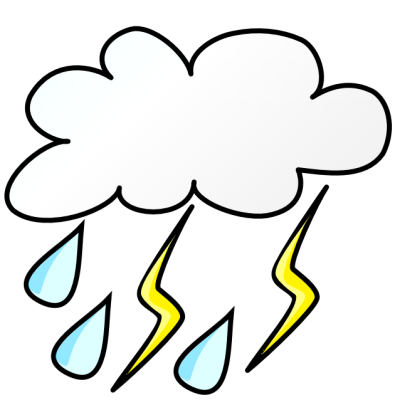
\includegraphics[width=0.2\textwidth]{./imagenes/tormenta.png} 
\caption{Nube de tormenta con rayos y lluvia}
\label{F:tormenta}
\end{figure}

La instrucción para insertar la gráfica es:


\begin{lstlisting}[]
\begin{figure}[H]
\centering
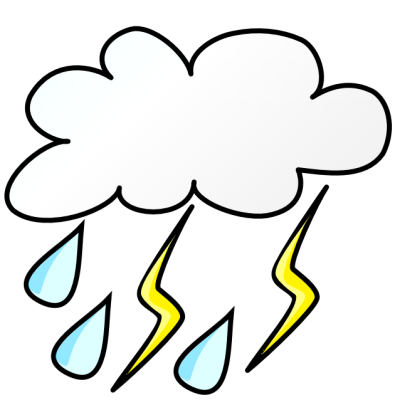
\includegraphics[width=0.2\textwidth]{./imagenes/tormenta.png} 
\caption{Nube de tormenta con rayos y lluvia}
\label{F:tormenta}
\end{figure}
\end{lstlisting}

La descripción es la siguiente:

\begin{itemize}\itemsep0pt \parskip0pt \parsep0pt
\item \verb+\begin{figure}[H]+ en la línea 1 inicia el entorno de la figura y declara que será ubicada inmediatamente luego del texto, con \verb+[H]+.
\item \verb+\centering+ en la línea 2 es una instrucción abreviada para indicar que la figura estará centrada.
\item \verb+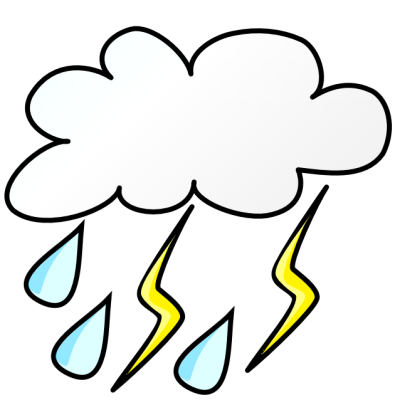
\includegraphics[width=0.2\textwidth]{./imagenes/tormenta.png}+ es la instrucción para insertar el archivo de la imagen, junto con indicaciones adicionales sobre el tamaño (un 20 \% del ancho del texto).
\item \verb+\caption{Nube de tormenta con rayos y lluvia}+ la instrucción  \texttt{caption}\footnote{En inglés, es bastante explícita esta instrucción, y en general puede decirse lo mismo de todos los comandos de \LaTeX, (ver por ejemplo \textsf{footnote}, \textsf{includegraphics}, \textsf{subsection}, etc.)} es el pie de figura con el nombre y la explicación. El número de figura lo inserta \LaTeX~ automáticamente.
\item \verb+\label{F:tormenta}+ es una etiqueta para referencia dentro de otras partes del texto.
\item \verb+\end{figure}+ cierra el entorno de la figura.
\end{itemize}

Como buena práctica, se recomienda nombrar el archivo de la imagen igual que la etiqueta, y con \textit{un nombre representativo}. Los nombres no deben tener espacios ni tildes ni eñes. Por ejemplo: \verb+senal_entrada_sinusoidal.jpg+.

\LaTeX, por defecto, va a ubicar las imágenes arriba o debajo de la página, y no inmediatamente después del texto en el que se escribe dentro del código, excepto que se indique lo contrario con \verb+\begin{figure}[h!]+ o con \verb+\begin{table}[H]+ utilizando el paquete \verb+float+.

Adicionalmente, se puede ubicar varias imágenes dentro de un mismo entorno de figura, como en la Figura \ref{F:subfiguras}. Ahí se muestran cuatro figuras distintas dentro del mismo entorno, donde se puede hacer referencia al transistor en \ref{F:subfig1}, al LED en \ref{F:subfig2}, al fotoconductor en \ref{F:subfig3} y al circuito integrado en \ref{F:subfig4}.

\begin{figure}[h!]
\centering
\subfloat[Transistor (texto que aparece en el índice)][Transistor en encapsulado TO-220]{
	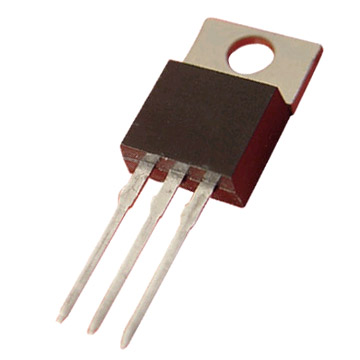
\includegraphics[width=0.2\textwidth]{./imagenes/transistor.jpg}
	\label{F:subfig1}}
\qquad
\subfloat[LED][LED blanco de baja potencia]{
	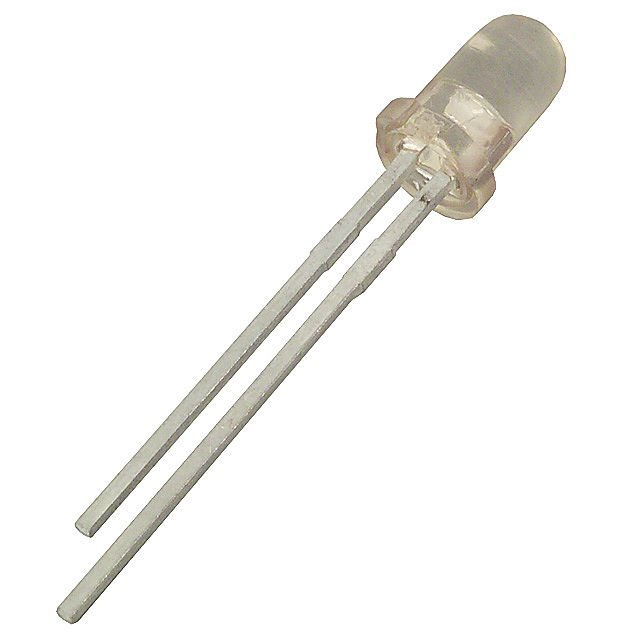
\includegraphics[width=0.2\textwidth]{./imagenes/led.jpg}
	\label{F:subfig2}}
\\
\subfloat[Fotoconductor][Fotoconductor]{
	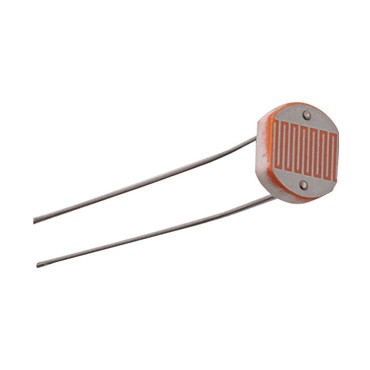
\includegraphics[width=0.2\textwidth]{./imagenes/fotoconductor.jpg}
	\label{F:subfig3}}
\qquad
\subfloat[Circuito integrado][Circuito integrado en encapsulado DIP-8]{
	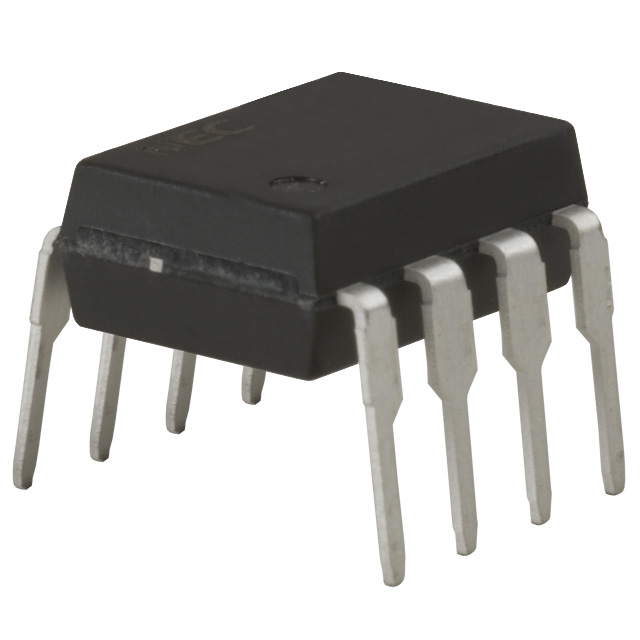
\includegraphics[width=0.2\textwidth]{./imagenes/integrado.jpg}
	\label{F:subfig4}}
\caption{Una figura con varias subfiguras, utilizando el paquete \texttt{subfig}}
\label{F:subfiguras}
\end{figure}

\subsection{Tablas}
%%%%%%%%%%%%%%%%%%%

Para las tablas se debe utilizar el entorno \verb+table+.

Aquí hay dos casos posibles:

\begin{description}

\item [Que la tabla debe construirse en \LaTeX] y en ese caso se debe usar el entorno \verb+tabular+, que a su vez se incluye dentro de \verb+table+.

\item [Que la tabla es en realidad una imagen] si fue generada por otro programa o fue escaneada, etc. Esta imagen entonces se incluye dentro del entorno \verb+table+ para que sea tratada como tal (y se numere como tabla, y se incluya en el índice de tablas, y se hagan las referencias como tablas, etc.).

\end{description}

Como ejemplo sencillo, la Tabla \ref{T:ejemplo} muestra una tabla con líneas verticales, declaradas como \verb+c | c+, que significa \textit{centrado - línea vertical - centrado}, y líneas horizontales, declaradas como \verb+\hline+ después de cada línea salto de línea (\verb+\\+).

\begin{table}
\caption{Comparación de velocidad de UWB con otros estándares alámbricos e inalámbricos}
\label{T:ejemplo}
\begin{center}
\begin{tabular}{ c | c}
\hline
\textbf{Velocidad [Mbits/s]} & \textbf{Estándar} \\ 
\hline
480 & UWB, USB 2.0 \\ 
200 & UWB (4 m) \\
110 & UWB (10 m) \\ 
90 & Fast Ethernet \\ 
54 & 802.11a \\ 
20 & 802.11g \\ 
11 & 802.11b \\ 
10 & Ethernet \\ 
3 & Bluetooth \\ 
0,256 & ZigBee \\ 
\hline
\end{tabular}
\end{center}
\end{table}

La instrucción \verb+\begin{tabular}{ | c | c |}+ genera un cuadro con líneas verticales en ambos lados, como en la Tabla \ref{T:ejemploconlineas}. 

Cuando se tiene un documento de dos o más columnas, es importante notar que una tabla puede ser muy grande y no quepa en una sola columna, por tanto debe especificarse que se acomode a todo lo ancho de la página. Esto es sencillo: basta con escribir \verb+table*+ al inicio y al final cuando se declara el entorno en \verb+\begin{} ... \end{}+.

\begin{table*}
\caption[Título en el índice]{Título que aparece en el pie de figura o encabezado de la tabla. Puede ser bastante amplio y explicar con más detalle. Debido a que el título que aparece en el índice es corto, no hay problema de que se exceda el espacio apropiado ahí.}
\label{T:ejemploconlineas}
\begin{center}
\begin{tabular}{| c | c |}
\hline
\textbf{Velocidad [Mbits/s]} & \textbf{Estándar} \\ 
\hline
480 & UWB, USB 2.0 \\ 
200 & UWB (4 m), 1394a (4,5 m) \\
110 & UWB (10 m) \\ 
90 & Fast Ethernet \\ 
54 & 802.11a \\ 
20 & 802.11g \\ 
11 & 802.11b \\ 
10 & Ethernet \\ 
3 & Bluetooth \\ 
0,256 & ZigBee \\ 
\hline
\end{tabular}
\end{center}
\end{table*}

Del mismo modo que en las figuras, \LaTeX~ por defecto colocará la tabla en la parte superior de la siguiente página, excepto que se indique lo contrario (con \verb+\begin{table}[h!]+)\footnote{Para mejor manejo de la posición de figuras, tablas y otros, utilizar el paquete \textsf{float}}.

\begin{table}
\caption{Otra tabla utilizando el paquete \texttt{booktabs}}
\label{T:otratabla}
\centering
\begin{tabular}{c l r r}
\toprule
\multicolumn{2}{c}{Producto} \\
\cmidrule(r){1-2}
Cantidad & Descripción & Precio unitario & Precio total  \\
\midrule
3  & Transistores 	& 250	& 750	\\
4  & Osciladores   	& 500   & 2000 \\
3  & Amp Ops     	& 600   & 1800	\\
10 & Resistores  	& 25    & 250	\\
10 & Capacitores	& 50 	& 500	\\
\midrule 
\multicolumn{3}{r}{TOTAL} & \textbf{5300} \\
\bottomrule
\end{tabular}
\end{table}

%%%%%%%%%%%%%%%%%%%%%%%%%%%%%
\section{Herramientas útiles}
%%%%%%%%%%%%%%%%%%%%%%%%%%%%%

%----------------------------------
\subsection{Referencias a figuras, tablas, ecuaciones, secciones y otros}

Es fundamental a lo largo del texto hacer referencias a figuras, tablas, ecuaciones, secciones y otros. Todos estos elementos tienen una etiqueta \verb+\label{}+ asociada a cada uno. 

La instrucción para hacer la referencia a esta etiqueta es \verb+\ref{}+.

Así entonces, se puede hacer referencia a las ecuaciones (\ref{E:desigualdad}), (\ref{E:anchodebanda}) y (\ref{E:fraccional}), a la Figura \ref{F:tormenta} y a la Tabla \ref{T:ejemplo} desde cualquier parte del texto, sin importar la numeración, que será asignada automáticamente por \LaTeX.

Es buena práctica nombrar las ecuaciones como \verb+\label{E:ecuacion}+, las tablas como \verb+\label{T:tabla}+, las figuras como \verb+\label{F:figura}+, y así sucesivamente, es decir, con una E, T, F o S antepuestas para identificar de qué se trata en cada caso, y con un nombre representativo. 

No es bueno hacer referencias relativas como ``la siguiente figura'' o ``la tabla anterior'' porque en realidad no se sabe la ubicación final dentro del texto. Hay que notar que tanto las tablas como las figuras, a menos de que se especifique lo contrario\footnote{Como se ha explicado, una forma de cambiar esto es colocando [h!] o [H] (de \emph{here}) junto al inicio del entorno.}, se colocarán al principio o al final de la página, en donde el programa lo considere mejor por motivo de espacio. Es mejor una referencia absoluta tal como figura \ref{F:tormenta} o ecuación (\ref{E:fraccional}). 

En editores de escritorio, algunas veces es necesario compilar dos o tres veces para que se carguen correctamente los números de referencia.

\subsection{Citas bibliográficas}
%%%%%%%%%%%%%%%%%%%%%%%%%%%%%%%%%

Los trabajos académicos requieren de referencias a las fuentes de información, invariablemente. Es necesario entonces considerar cómo crear una bibliografía y cómo referirse a las fuentes dentro del texto. 

Se puede hacer una bibliografía ``a mano'', en el que se le da la edición necesaria a cada entrada\footnote{En el código fuente de este documento hay un ejemplo de bibliografía tipo ``plain''.}. Sin embargo, BibTeX es una mejor alternativa, que permite administrar y modificar fácilmente una gran cantidad de entradas, además de que hace posible la reutilización de las referencias, en otros documentos.

\subsubsection{BibTeX}

\href{http://www.bibtex.org/}{BibTeX} es un programa de manejo de referencias. En este documento se utiliza de la siguiente forma:

\begin{itemize}
\item En un archivo llamado \texttt{bibliografia.bib} se introducen todas las referencias utilizadas, con el formato especial para ello. Ejemplo:
\begin{verbatim}
@BOOK {Valiente2001,
    author    = "Valiente Feruglio, G.",
    title     = "Composición de Textos Científicos con LaTeX",
    publisher = "Alfaomega",
    year      = "2001",
    address   = "México D.F.",
    edition   = "primera"
}
\end{verbatim}
Una buena herramienta para editar estas entradas se encuentra en \url{http://truben.no/latex/bibtex/}, sin embargo, considerar los sistemas de manejo bibliográfico de la siguiente sección.

\item Dentro del texto se hace referencia a las fuentes. La instrucción para hacer una cita es \verb+\cite{+\textit{clave}\verb+}+, dentro del cual se coloca la etiqueta, clave o \textit{key} asignada a la bibliografía (el primer espacio en la entrada de BibTeX de ejemplo), usualmente el apellido del primer autor y el año de publicación, por ejemplo: \verb+\cite{Valiente2001}+, que resulta en \cite{Valiente2001}.

\item Finalmente, al final del trabajo, se colocan las instrucciones 
\begin{verbatim}
\bibliographystyle{estilo}
\bibliography{nombrearchivo.bib}
\end{verbatim}
donde \texttt{estilo} es uno de los varios formatos posibles para las citas y las referencias (ver una lista en \url{https://www.sharelatex.com/learn/Bibtex_bibliography_styles}), y la segunda instrucción se encarga de colocar el título, y todas las entradas \textbf{que han sido citadas}, en el orden y el formato necesarios. Ahí es donde la ventaja de BibTeX se hace más evidente. 

\item En programas de edición de escritorio (Texmaker,\ldots) es necesario compilar varias veces y en una secuencia específica para que se genere la bibliografía. Esta secuencia es: \texttt{latex} \textgreater~ \texttt{bibtex} \textgreater~ \texttt{latex} \textgreater~ \texttt{latex}. En las plataformas de edición en línea (Overleaf,\ldots) esto se hace automáticamente.
\end{itemize}

\subsubsection{Sistemas de manejo bibliográfico}

En trabajos de investigación es necesario recurrir a muchas referencias (en tesis y otros, fácilmente más de 50) y el manejo de estas se puede tornar engorroso. Actualmente, varias plataformas ofrecen un manejo automatizado y muy conveniente de referencias. A continuación se presentan algunas opciones.

\begin{multicols}{2}
\begin{description}
\item[Mendeley] \url{http://www.mendeley.com/}
\item[Readcube] \url{http://www.readcube.com/}
\item[Docear] \url{http://www.docear.org/}
\item[Citavi] \url{http://www.citavi.com/}
\item[EndNote] \url{http://endnote.com/}
\item[JabRef] \url{http://jabref.sourceforge.net/}
\end{description}
\end{multicols}

\subsection{Formato}
%%%%%%%%%%%%%%%%%%%%

%---------------------------------------
\subsubsection{Cambiar el tipo de letra}

La tipografía de \LaTeX~ por defecto es la \href{https://en.wikipedia.org/wiki/Computer_Modern}{Computer Modern}. Es fácil de identificar y ampliamente utilizada (por la popularidad de \LaTeX) en muchas publicaciones científicas.

Esta plantilla de Proyecto Eléctrico utiliza la tipografía \href{http://www.linuxlibertine.org/}{Libertine}. 

Es útil, sin embargo, cambiar de tipografía en todo el documento o en algunas secciones\footnote{¡Cuidado! Demasiada libertad para cambiar el formato del documento puede derivar en malas decisiones de diseño gráfico. Ejemplo usual: utilizar Comic Sans (no disponible aquí).}.

Una referencia de la mayoría de tipografías disponibles para \LaTeX~ se encuentra en \url{http://www.tug.dk/FontCatalogue/}. Por ejemplo, la siguiente instrucción en el preámbulo convierte todo el texto a DejaVu Sans.

\begin{verbatim}
\usepackage{DejaVuSans}
\renewcommand*\familydefault{\sfdefault} 
\usepackage[T1]{fontenc}
\end{verbatim}

La instrucción \verb+{\fontfamily{qag}\selectfont ...texto...}+ genera {\fontfamily{qag}\selectfont un texto en otra tipografía. Para restringir la selección, el texto debe estar rodeado por llaves}. El código \texttt{qag} representa el tipo de letra. Una lista de tipos de letras y sus códigos, junto con más opciones se puede encontrar \href{https://www.sharelatex.com/learn/Font_typefaces}{aquí} y \href{http://tex.stackexchange.com/questions/25249/how-do-i-use-a-particular-font-for-a-small-section-of-text-in-my-document}{aquí}.

%-----------------------
\subsubsection{Unidades}

Las unidades deben escribirse separadas de la magnitud. Cuando se hace en una ecuación se presenta el problema que muestra la ecuación (\ref{E:sinunidades}). Para resolver este problema hay que incluir algún paquete que permita introducir unidades correctamente. En este documento se eligió \verb+siunitx+. La ecuación (\ref{E:conunidades}) muestra el uso corregido de las unidades en las ecuaciones. Del mismo modo, se puede poner de ejemplo: $C_s = \SI{0.1}{\micro\farad}$, $T_c = \SI{27}{\degreeCelsius}$. 

\begin{equation}\label{E:sinunidades}
{V}_{i}\ge 1,3 mV
\end{equation}

\begin{equation}\label{E:conunidades}
{V}_{i} \ge 1,3~\si{\milli\volt}
\end{equation}

O también el siguiente ejemplo:

\begin{equation}\label{E:unidades}
V = I_L \times R_L = \left( 0,25~\si{\milli\ampere} \right) \times \left( \SI{4}{\kilo\ohm} \right) = 1~\si{\volt} 
\end{equation}

%--------------------------------------------
\subsubsection{Otras herramientas de formato}

\begin{enumerate}
\item Las notas de pie\footnote{Que se insertan escribiendo la instrucción inmediatamente después del texto a comentar, como en este caso.}, utilizando la instrucción \verb+\footnote{}+.
\item Las comillas, que colocan con estos símbolos ``especiales'' y no las comillas del teclado. 
\item La palabra \LaTeX~ se escribe con el comando \verb+\LaTeX+. Debe escribirse el símbolo \verb+~+ después de la instrucción para que genere un espacio adecuado entre palabras, de otro modo \LaTeX queda pegado.
\item Las \textbf{negritas} se escriben con el comando \verb+\textbf{}+ (de \textit{\textbf{b}old \textbf{f}ace})
\item Las \textit{cursivas} se escriben con el comando \verb+\textit{}+ (de \textit{\textbf{it}alics})
\item Las \textsc{versales} se escriben con el comando \verb+\textsc{}+ (de \textit{\textbf{s}mall \textbf{c}aps})
\item Las \texttt{monoespacio} se escriben con el comando \verb+\texttt{}+ (de \textit{\textbf{t}ele\textbf{t}ype})
\item El comando \verb+\emph{}+ se utiliza para \emph{resaltar} un texto, muy similar a \verb+\textit{}+, con la diferencia que \textit{el resaltado depende del \emph{contexto} del párrafo}.
\item Hay varios tamaños de guiones: -, -- (con \verb+--+) y --- (con \verb+---+).
\item Se puede especificar la fecha de hoy, \today, utilizando el comando \verb+\today+.
\item El paquete \verb+hyperref+ permite la inclusión de hipervínculos, tanto a lugares externos del documento como internos (observe las referencias a tablas, figuras o ecuaciones o las citas bibliográficas). También incorpora los   marcadores que se muestran en los lectores de pdf y que se utilizan para navegación del documento. Por ejemplo, se puede hacer referencia a la Sección \ref{S:Figuras} donde se explica la inclusión de figuras (y hacer clic al hipervínculo y seguirlo).
\item Las listas numeradas (como esta) se hacen con el entorno \verb+\begin{enumerate}+, las listas con viñetas utilizando \verb+\begin{itemize}+.
\item Se pueden crear comandos especiales para insertar textos o símbolos definidos por el usuario. La instrucción es \verb+\newcommand{\comando}{Texto a introducir}+.
\item Por ejemplo, si no se quiere escribir cada vez ``Escuela de Ingeniería Eléctrica'' y además se le quiere dar un formato especial, entonces se puede indicar en el preámbulo 

\verb+\newcommand{\EIEx}{\textsc{Escuela \Lightning~ Ingeniería Eléctrica}}+ 

y así se crea el comando \verb+\EIEx+ que genera: \EIEx.
\item[--] Se puede utilizar un guión (o cualquier símbolo) en lugar de la numeración o las viñetas en una lista, con la instrucción \verb+[-]+ al lado de \verb+\item+.
\item[\Biohazard] Ejemplo de símbolo como viñeta\footnote{Las instrucciones \texttt{Lightning} y \texttt{Biohazard} son parte del paquete de símbolos especiales \texttt{marvosym}.}.
\end{enumerate}

\subsection{Figuras con PGF/Ti\textit{k}Z}
%%%%%%%%%%%%%%%%%%%%%%%%%%%%%%%%%%%%%%%%%%

PGF/Ti\textit{k}Z es un conjunto de lenguajes para producir gráficos vectoriales a partir de una descripción geométrica y algebraica\footnote{Tomado de su descripción en Wikipedia.}. Tiene grandes capacidades y una documentación exhaustiva.

La Figura \ref{F:tikz} es un ejemplo relativamente sencillo de las capacidades de Ti\textit{k}Z.

\begin{figure}[H]
\centering
	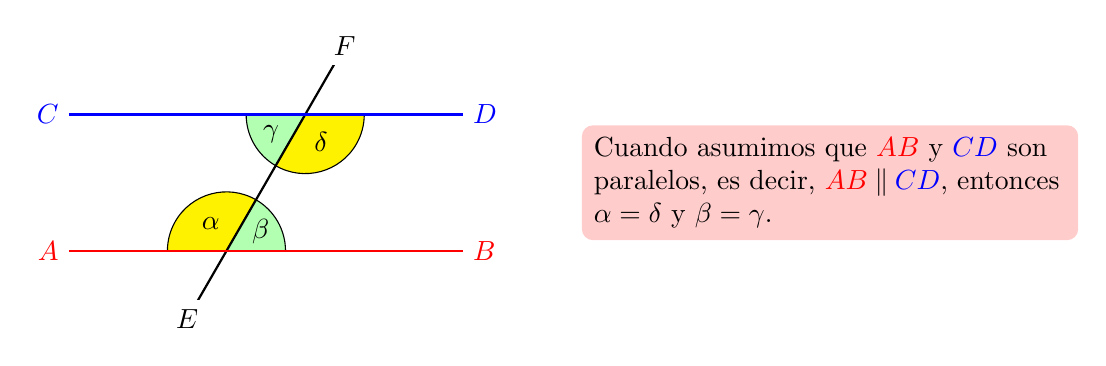
\begin{tikzpicture}
	  \draw[fill=yellow] (0,0) -- (60:.75cm) arc (60:180:.75cm);
	  \draw(120:0.4cm) node {$\alpha$};
	  \draw[fill=green!30] (0,0) -- (right:.75cm) arc (0:60:.75cm);
	  \draw(30:0.5cm) node {$\beta$};
	  \begin{scope}[shift={(60:2cm)}]
	    \draw[fill=green!30] (0,0) -- (180:.75cm) arc (180:240:.75cm);
	    \draw (30:-0.5cm) node {$\gamma$};
	    \draw[fill=yellow] (0,0) -- (240:.75cm) arc (240:360:.75cm);
	    \draw (-60:0.4cm) node {$\delta$};
	  \end{scope}
	  \begin{scope}[thick]
	    \draw  (60:-1cm) node[fill=white] {$E$} -- (60:3cm) node[fill=white] {$F$};
	    \draw[red]                   (-2,0) node[left] {$A$} -- (3,0) node[right]{$B$};
	    \draw[blue,shift={(60:2cm)}] (-3,0) node[left] {$C$} -- (2,0) node[right]{$D$};
	    \draw[shift={(60:1cm)},xshift=4cm]
	    node [right,text width=6cm,rounded corners,fill=red!20,inner sep=1ex]
	    {
	      Cuando asumimos que $\color{red}AB$ y $\color{blue}CD$ son paralelos, es decir, ${\color{red}AB} \mathbin{\|} \color{blue}CD$, entonces $\alpha = \delta$ y $\beta = \gamma$.
	    };
	  \end{scope}
	\end{tikzpicture}
\caption[Ejemplo de uso de PGF/Ti\textit{k}Z]{Ejemplo de uso de PGF/Ti\textit{k}Z, pero solo una muestra de sus capacidades.}
\label{F:tikz}
\end{figure}

Una buena cantidad de ejemplos están disponibles en \url{http://www.texample.net/tikz/} y la documentación (incluyendo un manual de uso de más de 700 páginas) está en \url{https://www.ctan.org/pkg/pgf?lang=en}.

%---------------------------------------
\subsection{Gráfico de datos y funciones con \texttt{pgfplots}}

%---------------------------------------
\subsection{Circuitos con Circuitikz}

El paquete \texttt{circuitikz} permite la creación de circuitos eléctricos y electrónicos. La Figura \ref{F:ampop} es un ejemplo.

\begin{figure}
  	\centering
		 \begin{circuitikz}[american]
		  \draw
		  % El amplificador operacional
		  (0,0) node[op amp] (opamp) {} node[] {{\tiny Amp Op}}
		  
		  % Las entradas
		  (opamp.-) node[circ] {} to[R, l_=$R_1$] ++(-2,0) node[ocirc] {} node[left] {$V_{s}$}
		  (opamp.+) -- ++(0,-0.5) node[ground] {} 
		  
		  % El lazo de realimentación
		  (opamp.-) -- ++(0,1)  to[R, l=$R_2$] ++(2,0) -| (opamp.out) {}
		  
		  % La salida
		  (opamp.out) -- ++(0.5,0) node[circ] {} to[R, l=$R_L$] ++(0,-2) to [short, i_=$I_o$] ++(0,0) node[ground] {}
		  (opamp.out) -- ++(1,0) node[ocirc] {} node[right]{$V_o$}
		  
		  ;
		\end{circuitikz}
    \caption[Amplificador inversor]{Amplificador inversor con un amplificador operacional cuya relación entrada--salida está dada por $V_o = -\frac{R_2}{R_1} V_s$.}
    \label{F:ampop}
\end{figure}

\begin{figure}
\centering
\begin{circuitikz}
\draw
	(0,0)
    	to [V, l=50~\si{\volt}] (0,2) to (0,3)
        to [R, l=$20~\si{\kilo\ohm}$] (5,3) to (5,2)
        to [vR, l=$R$] (5,0)
        to (0,0)
  	(0,2)
    	to [R, l_=$5~\si{\kilo\ohm}$] (5,2)     
;
\end{circuitikz}
\caption{Circuito básico.}
\label{F:circuitobasico}
\end{figure}

\begin{figure}
\centering
\begin{circuitikz}
\draw
	(0,0) node[ground]{}
    	to [V, l=(``Arenal'') $V_{1}$] (0,3)
        to [short] (0.5,3) node[circ]{}
   	(5.5,3)
        to [short] (5.5,4)
        to [R, l=$R_{1}$, i<=$I_{1}$] (3,4)
        to [cV, l=$v_{1}$] (0.5,4)
        to [short] (0.5,3)   
   	(6,3)
    	to [short] (5.5,3)
        to [short] (5.5,2)
        to [R, l=$R_{3}$, i<=$I_{2}$] (3,2)
        to [cV, l=$v_{3}$] (0.5,2)
        to [short] (0.5,3)
	(6,3) node[circ]{}
    	to [generic, i_=$I_{L}$, v^=$v_{L}$] (6,0) node[ground]{}
   	(6,3)
    	to [R, l=$R_{2}$, i<=$I_{3}$] (8.5,3)
        to [cV, l=$v_{2}$] (11,3)
    (11,0) node[ground]{}
        to [V, l_=$V_{2}$ (``Miravalles'')] (11,3)
;
\end{circuitikz}
\caption[Circuito de transmisión de potencia]{Circuito de transmisión de potencia por varias líneas conductoras desde centros de generación y con sistemas de ajuste de la corriente.}
\label{F:transmisionpotencia}
\end{figure}

\begin{figure}
\centering
\begin{circuitikz}
\draw 
(0,0)	to [battery, l_=$V_i$] (0,3)
		to [R, l_=$R_1$] (2.5,3)
        to [cV, l_=$A v_x$] (5,3)
        to [short] (6,3)
        to [vR, l_=$R_T$, i=$i_{R_T}$] (6,0) node[ground]{}
        to [short] (0,0)
(6,3)	to [short] (7,3)
(6,0)	to [short] (7,0)

;
\draw (2.5,3) to [open, v=$v_x$] (2.5,0);
\draw (2.5,3) node[circ]{};
\draw (2.5,0) node[circ]{};

\draw[dashed] (-0.8,-0.8) rectangle (4.8,3.8);
\draw (-0.8,-0.8) node [above right]{Fuente de corriente};

\draw (7,-0.5) rectangle (9,3.5);
\draw (8,1.5) node [align=center]{Circuito \\ de acople};

\draw 
(9,3)	to [short] (10,3)
		to [R, l_=$R_2$] (12,3)
		to [generic, l_=$Y$, v^=$v_Y$] (14,3)
(9,0)   to [short] (14,0) node[ground]{}
		to [cV, l=$A v_z$] (14,3)
(14,0)	to [short] (15.3,0)
		to [open, v>=$v_o$] (15.3,3)
		to [short] (14,3)
;
\draw (12,3)	to [open, v=$v_z$] (12,0);
\draw (12,3) node[circ]{};
\draw (12,0) node[circ]{};

\draw[dashed] (9.8,-0.8) rectangle (14.8,3.8);
\draw (9.8,-0.8) node [above right]{Amplificador};

\draw (15.3,3) node[circ]{} node[right]{$a$};
\draw (15.3,0) node[circ]{} node[right]{$b$};
\end{circuitikz}
\caption[Circuito de acondicionamiento y amplificación]{Circuito de acondicionamiento y amplificación de la señal de un sensor resistivo $R_T$, dependiente de la temperatura.}
\label{F:acondicionamiento}
\end{figure}

\begin{figure}
\centering
\begin{circuitikz}

% PNP Q1
\draw
	(0,4) 	node[pnp,rotate=90](Q1){} node[above]{$Q_1$}
;
% NPN Q2
\draw
	(0,1.5) 	node[npn,rotate=180,yscale=-1](Q2){} node[left]{$Q_2$}
;
% Op Amp
\draw
	(3,1.5) 	node[op amp,rotate=180,yscale=-1](CMP){} node[]{AMP}
;
% Resistores
\draw
	(6,4) node[circ]{} 
    	to [R, l=$R_1$] (6,2) 
    	to [R, l=$R_2$] (6,0) node[ground]{}
;
% Conectores
\draw
	(-1.5,4) 	node[ocirc]{} node[above]{$V_{IN}$} 
    		to [short] (Q1.emitter)
  	(Q1.base) to [short] (Q2.collector)
    (Q2.emitter) to [short] (0,0) node[ground]{}
    (CMP.out) to [short] (Q2.base)
    (Q1.collector) to [short] (7,4) node[ocirc]{} node[above]{$V_{OUT}$}
    (CMP.-) to [short] (6,2) node[circ]{}
    (4.5,0) node[ground]{} to [battery,l_=$V_{R}$] (4.5,1) to [short] (CMP.+) 
;
\end{circuitikz}
\caption{Regulador lineal de tensión con lazo de control.}
\label{F:reguladorlineal}
\end{figure}

\begin{figure}
\centering
\begin{circuitikz} 
\draw
	(0,0) node[op amp,yscale=-1] (opamp) {}
    (0,0) node[](){CMP}
;

\draw 
	(-4.5,2) node[rground, yscale=-1](){} 
    to [I, l_=$I$] (-4.5,1)
    to [short,-*] (-4.5,0.5)
    to [short] (-4.5,-1.8) 
;

\draw 
	(-3,2) node[rground, yscale=-1](){} 
    to [I, l_=$I$] (-3,1)
    to [short,-*] (-3,-0.5) 
    to [R, l_=$R_1$] (-3,-2.5)
    to [R, l_=$R_2$] (-3,-4.5) node[ground](){}
;

\draw 
	(-3,-2.5) to [short,*-] (-2,-2.5)
    to [cspst,] (-2,-4.5) 
    to [short] (-3,-4.5)
    (-1.8,-3.8) node[right](){SW}
;

\draw 
	(-4.5,-2.5) node[pnp](pnp){}
	(pnp.base) node[anchor=east] {\tiny{B}}
    to [short] (-5.3,-4.5) to [short,-*] (-4.5,-4.5)
    (pnp.emitter) node[anchor=east]{\tiny{E}} 
    (pnp.collector) node[anchor=east] {\tiny{C}}
    to [short] (-4.5,-4.5) to [short,-*] (-3,-4.5)
    (-4.5,-2.5) node[anchor=west] {$Q_T$}
;

\draw (opamp.-) to [short] (-3,-0.5) node[anchor=east]{$V^-$};
\draw (opamp.+) to [short] (-4.5,0.5) node[anchor=east]{$V^+$};
\draw (opamp.out) to [short] (1.5,0);
\draw[dashed] (1.5,0) -- (1.5,-3.4) -- (-1.7,-3.4);

\draw (4,0)  node[ocirc]{} node[anchor=south]{\={S}} to [full diode] (1.5,0) node[circ]{} node[anchor=south]{$V_{\mathrm{CMP}}$};

\end{circuitikz}
\caption{Circuito para protección térmica con lazo de histéresis.}
\label{F:protecciontermica}
\end{figure}

\subsection{Inserción de código fuente}
%%%%%%%%%%%%%%%%%%%%%%%%%%%%%%%%%%%%%%%

En ocasiones es necesario introducir secciones de código fuente de programación dentro de reportes. La inserción es especial, pues el compilador no debe confundir las instrucciones dentro del código con instrucciones de \LaTeX. Además, se prefiere un formato específico con resaltado de sintaxis para mejorar la legibilidad (como en los editores de código o en los IDE). Un paquete que provee soluciones para este requisito es \texttt{listings}.

Para el código fuente hecho en Matlab es posible utilizar el paquete \texttt{mcode} (adjunto como archivo a la carpeta que contiene el proyecto) que asigna a \texttt{listings} el formato apropiado, como se ve en el siguiente código:

\lstinputlisting[inputencoding=latin1]{codigo/codigoejemplo.m}

%%%%%%%%%%%%%%%%%%%%%%%%%%%%%%%%%
\section{Referencias para \LaTeX}
%%%%%%%%%%%%%%%%%%%%%%%%%%%%%%%%%

La comunidad de usuarios de \LaTeX~ es grande y colaborativa. Hay multitud de recursos en línea para aprender buenas prácticas y ``trucos'' para mejorar los documentos. Algunas de las mejores referencias son:

\begin{description}
\item[Wikibook] \url{https://en.wikibooks.org/wiki/LaTeX}
\item[Cookbook] \url{http://latex-cookbook.net/}
\item[TeXample] \url{http://texample.net/}
\item[HowtoTeX] \url{http://www.howtotex.com/}
\item[Font Catalogue] \url{http://www.tug.dk/FontCatalogue/}
\end{description}

\subsection{¿Dónde editar \LaTeX?}\label{S:programas}
%%%%%%%%%%%%%%%%%%%%%%%%%%%%%%%%%%%%%%%%%%%

\paragraph{Editores de texto ``de escritorio''}

Existen varios programas para la edición y compilación de archivos de \LaTeX. Se ha escogido Texmaker debido a que es multiplataforma (Mac, Linux, Windows) y cuenta con otras características como resaltado de sintaxis, autocompletar, corrección ortográfica, asistente para la creación de documentos, accesos rápidos a símbolos, comandos y entornos, entre otros. Se puede, claro está, editar el documento con cualquier editor y compilar, siempre y cuando se tengan los paquetes necesarios\footnote{Esta es una ventaja de ser un código estándar abierto.}.

En Windows, junto con Texmaker debe instalarse MiKTeX, que es un conjunto de paquetes, fuentes y demás necesarios para compilar el archivo.

Ambos están disponibles para descarga gratuita desde \url{http://miktex.org/} y \url{http://www.xm1math.net/texmaker/}.

Una base de datos extensiva de los paquetes de \LaTeX~ está en \url{http://www.ctan.org/}. Es especialmente útil para encontrar la documentación de los paquetes. Desde esta página se pueden descargar los paquetes, pero la mejor forma de revisar los paquetes disponibles e instalarlos fácilmente es a través del \emph{MiKTeX Package Manager}, disponible después de instalar el MiKTeX.

\paragraph{Plataformas en línea de edición para \LaTeX}

Una alternativa muy popular de años muy recientes es la edición en línea. Entre las ventajas se encuentran: almacenamiento en línea, edición colaborativa, herramientas web (bibliografías y otros), compilación simultánea, más la mayoría de las otras ventajas de los editores ``de escritorio'' como autocompletar, símbolos, etc.

Los editores más populares son:

\begin{description}
\item[Overleaf] \url{https://www.overleaf.com/}
\item[ShareLaTeX] \url{https://www.sharelatex.com/}
\item[Papeeria] \url{https://papeeria.com/}
\end{description}
%% ----------------------------------------
  \chapter{Conclusiones y recomendaciones}
% ----------------------------------------
\label{C:conclusiones}

El informe debe terminarse con la enumeración de las principales conclusiones derivados del trabajo realizado.  En particular, debe verificarse el cumplimiento de los objetivos planteados para el mismo.

\section{Conclusiones}
El aporte (\emph{novedad}) hecho con el proyecto, debe destacarse.

Las conclusiones pueden enumerarse en forma suscinta como una lista, ya sea itemizada o numerada.

\section{Recomendaciones}
Con base en las trabajo realizado y las conclusiones sobre el mismo, puede ser necesario incluir una sección, o lista, de recomendaciones.  Por ejemplo, sobre la utilización de otro enfoque para resolver el problema.

% 9. APÉNDICES
% ------------
\appendix
\chapter{Páginas de la 7 a la 25 de la norma INTE 31-08-06-2000}
\label{A}


\includepdf[pages=7-25]{./imagenes/Inteco.pdf}


%\begin{figure}[H]
%	\centering
%	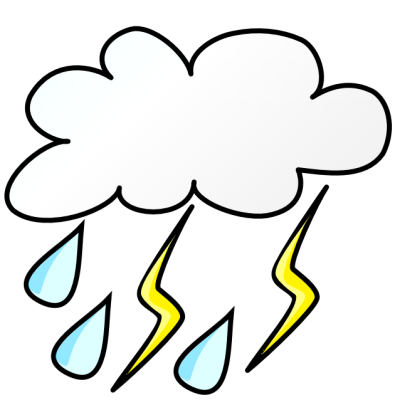
\includegraphics[width=0.2\textwidth]{./imagenes/tormenta.png} 
%	\caption{Nube de tormenta con rayos y lluvia}
%	\label{F:tormenta}
%\end{figure}
\chapter{Otro apéndice de ejemplo}
\label{B}

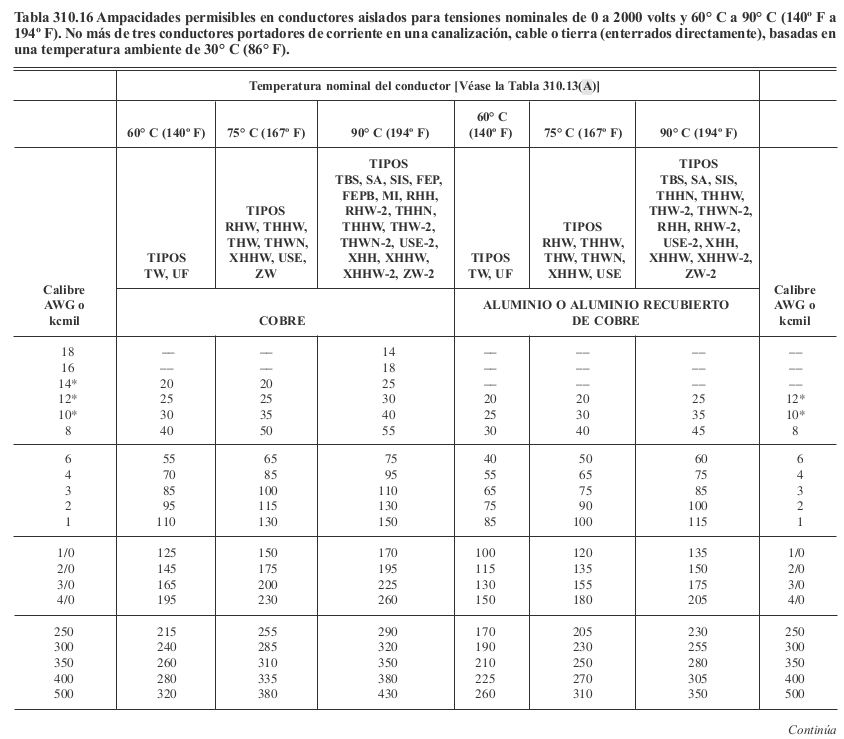
\includegraphics[width=1\textwidth]{./imagenes/cable1.png} 

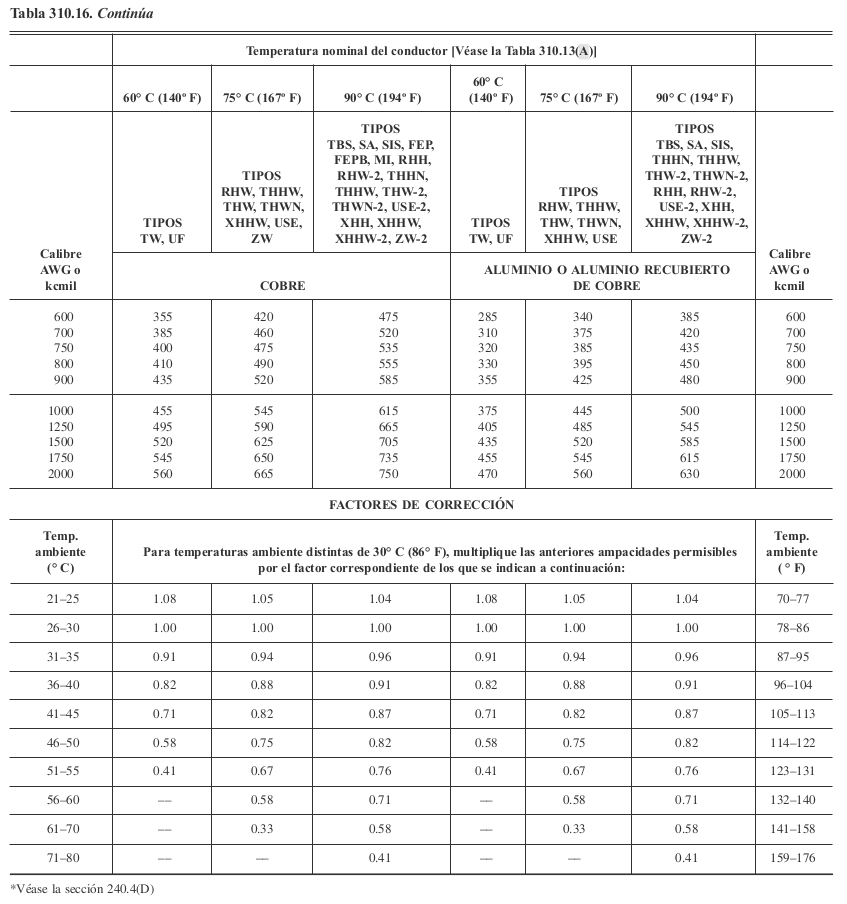
\includegraphics[width=1\textwidth]{./imagenes/cable2.png} 

\backmatter

% 10. BILIOGRAFÍA
% --------------
\bibliographystyle{plain}
\bibliography{contenido/bibliografia.bib}

%%%%%%%%%%%%%%%%%%%
\end{document}
%%%%%%%%%%%%%%%%%%%
